% =============================================================================
%  Capítulo 3: Programación Lineal
%  Basado en:
%    Steven L. Brunton, "Optimization: A Bootcamp for Machine Learning,
%    Inverse Problems, and Control", Cambridge University Press, 2026.
%    Capítulo 3, secciones 3.1--3.6 (pp. 89-121).
%
%  Contenido verificado del capítulo:
%    3.1 Problem Statement and Examples
%    3.2 Polytopes, Vertices, and High-Dimensional Geometry
%    3.3 Dantzig's Simplex Method
%    3.4 Simplex Tableau Method
%    3.5 Duality in Linear Programming
%    3.6 Integer Programming and NP-Hard Problems
%
%  Compilar:  make
% =============================================================================

\documentclass[10pt,aspectratio=169]{beamer}

% --- Idioma y codificación ---------------------------------------------------
\usepackage[utf8]{inputenc}
\usepackage[T1]{fontenc}
\usepackage[spanish]{babel}

% --- Matemáticas -------------------------------------------------------------
\usepackage{amsmath,amssymb,mathtools}

% --- Tablas y diseño ---------------------------------------------------------
\usepackage{booktabs}
\usepackage{tabularx}
\usepackage{array}
\usepackage{lmodern}
\usepackage{microtype}

% --- Colores -----------------------------------------------------------------
\definecolor{unah}{RGB}{0,82,155}
\definecolor{acento}{RGB}{0,135,110}

\setbeamercolor{structure}{fg=unah}
\setbeamercolor{frametitle}{fg=unah}
\setbeamercolor{itemize item}{fg=acento}
\setbeamercolor{itemize subitem}{fg=unah}
\setbeamertemplate{itemize item}{\color{acento}\scriptsize$\blacktriangleright$}
\setbeamertemplate{itemize subitem}{\color{unah}\scriptsize$\bullet$}

% --- Plantillas --------------------------------------------------------------
\setbeamertemplate{navigation symbols}{}
\setbeamertemplate{footline}[frame number]

% --- Fuente de las figuras ---------------------------------------------------
\newcommand{\fuente}{\vfill{\scriptsize\color{gray}Brunton, \emph{Optimization Bootcamp}, Cap.~3}}

\title{Cap. 3: Programación Lineal}

% =============================================================================
\begin{document}
% =============================================================================

% --- Portada -----------------------------------------------------------------
\begin{frame}
  \titlepage
\end{frame}

% --- Esquema -----------------------------------------------------------------
\begin{frame}{Temas de Programación Lineal}
  \tableofcontents
\end{frame}

% =============================================================================
\section{¿Qué es un programa lineal?}
% =============================================================================

\begin{frame}{El problema central}
  \small
  \begin{itemize}
    \item Hasta aquí: optimización \emph{sin restricciones}.
    \item La \textbf{programación lineal (PL)}: problemas \emph{convexos con restricciones},
      con función objetivo \emph{lineal}.
    \item Nace de recursos limitados (tiempo, espacio, dinero, materiales), que producen
      \emph{tradeoffs} expresados como desigualdades.
    \item Se desarrolló en la Segunda Guerra Mundial (racionamiento y logística).
    \item Sin solución analítica en forma cerrada, pero con algoritmos exactos que escalan
      a miles de variables y restricciones.
  \end{itemize}
  \begin{block}{Forma estándar}
    \[\max_x\; c^T x \quad \text{s.t.}\quad Ax \le b,\qquad x \ge 0\]
    $c \in \mathbb{R}^n$, $A \in \mathbb{R}^{m\times n}$, $b \in \mathbb{R}^m$.
  \end{block}
  \fuente
\end{frame}

\begin{frame}{La geometría lo determina todo}
  \small
  \begin{itemize}
    \item Cada restricción $a_j^T x \le b_j$ es un \textbf{semi-espacio}; el conjunto
      factible es la intersección de semiplanos con el cuadrante positivo:
      un \textbf{polítopo convexo}.
    \item El objetivo lineal es a la vez convexo y cóncavo: tanto maximizar como
      minimizar son tareas \textbf{convexas}.
    \item El gradiente del objetivo es \emph{constante}: $\nabla f(x) = c$.
    \item \textbf{El óptimo siempre ocurre en un vértice} del politopo.
    \item \textbf{Óptimo local $=$ óptimo global}: al ser convexo, basta encontrar un
      extremo local.
  \end{itemize}
  \begin{alertblock}{El problema combinatorio}
    Un hipercubo de dimensión $n$ tiene $2^n$ vértices: $2^{20}$ supera el millón.
    Enumerar vértices es intratable $\Rightarrow$ hace falta un algoritmo de búsqueda
    eficiente: el \textbf{simplex}.
  \end{alertblock}
  \fuente
\end{frame}

\begin{frame}{Ejemplo: la fábrica de microscopios}
  \small
  Ganancia \$100 (enseñanza) y \$400 (investigación); capacidad total 50/mes;
  demanda máxima de investigación 30/mes.
  \[
    \max_{x_1,x_2}\; 100 x_1 + 400 x_2 \quad \text{s.t.}\quad
    x_1+x_2 \le 50,\;\; x_2 \le 30,\;\; x_1,x_2 \ge 0
  \]
  \begin{columns}[T,onlytextwidth]
    \begin{column}{.46\textwidth}
      \small
      \begin{tabularx}{\textwidth}{@{}l l r@{}}
        \toprule
        Vértice & $(x_1,x_2)$ & $f$ \\
        \midrule
        $v_1$ & $(0,0)$   & $0$ \\
        $v_2$ & $(50,0)$  & $5000$ \\
        $v_3$ & $(0,30)$  & $12000$ \\
        $v_4$ & $(20,30)$ & $\mathbf{14000}$ \\
        \bottomrule
      \end{tabularx}
    \end{column}
    \begin{column}{.5\textwidth}
      \small
      \begin{block}{En Python}
        \small
        \texttt{pulp}: \texttt{LpMaximize}, \texttt{LpVariable}, \texttt{solve()}.
        \medskip
        Da $x_1 = 20$, $x_2 = 30$, profit $14000$.
      \end{block}
    \end{column}
  \end{columns}
  \fuente
\end{frame}

% =============================================================================
\section{Polítopos, vértices y holgura}
% =============================================================================

\begin{frame}{Geometría de los politopos}
  \small
  \begin{itemize}
    \item Cada frontera del politopo la define una desigualdad \textbf{activa}
      (\emph{tight}), que se comporta como una igualdad.
    \item Cada \textbf{vértice} es la intersección de $n$ fronteras activas en $n$ dimensiones.
    \item Para acotar un politopo en $n$ dimensiones hacen falta al menos $n+1$
      superficies $(n-1)$-dimensionales.
    \item Vértices adyacentes están unidos por una arista unidimensional.
  \end{itemize}
  \begin{block}{Variables de holgura}
    \[
      \max_x\; c^T x \quad \text{s.t.}\quad Ax + s = b,\qquad x, s \ge 0
    \]
    $s_i$ cuantifica la distancia a la frontera $i$:
    \textbf{$s_i = 0$ $\Rightarrow$ la restricción $i$ está activa.}
    Un punto interior tiene todas las holguras estrictamente positivas.
  \end{block}
  \vfill
  {\scriptsize\color{gray}
    Sinónimos en la literatura: variables \emph{tight} $=$ no básicas;
    variables \emph{slack} $=$ básicas.}
  \fuente
\end{frame}

\begin{frame}{Arrancando el Método Simplex}
    \framesubtitle{?`Cómo hallar el primer vértice?}
  \small
  \begin{columns}[T,onlytextwidth]
    \begin{column}{.48\textwidth}
      \textbf{Encontrar un vértice (desde cero)}
      \begin{itemize}
        \item $n$ restricciones activas $\Rightarrow$ sistema lineal
          $\tilde{A}x = \tilde{b}$.
        \item Se resuelve por inversión de matriz:
          coste $\mathcal{O}(n^3)$.
        \item Prohibitivo en dimensiones altas.
      \end{itemize}
    \end{column}
    \begin{column}{.48\textwidth}
      \textbf{Caminar a un vértice vecino}
      \begin{itemize}
        \item Basta \emph{tensar} una holgura y \emph{aflojar} una tight.
        \item Se intercambia un solo par de variables.
        \item Mucho más barato: es la \textbf{base del simplex}.
      \end{itemize}
    \end{column}
  \end{columns}
  \vfill
  \begin{block}{Idea clave}
    No se resuelven vértices: se camina de vértice en vértice, cambiando una
    restricción activa por una inactiva en cada paso.
  \end{block}
  \fuente
\end{frame}

\begin{frame}{La región factible y sus vértices}
  \small
  \begin{figure}
    \centering
    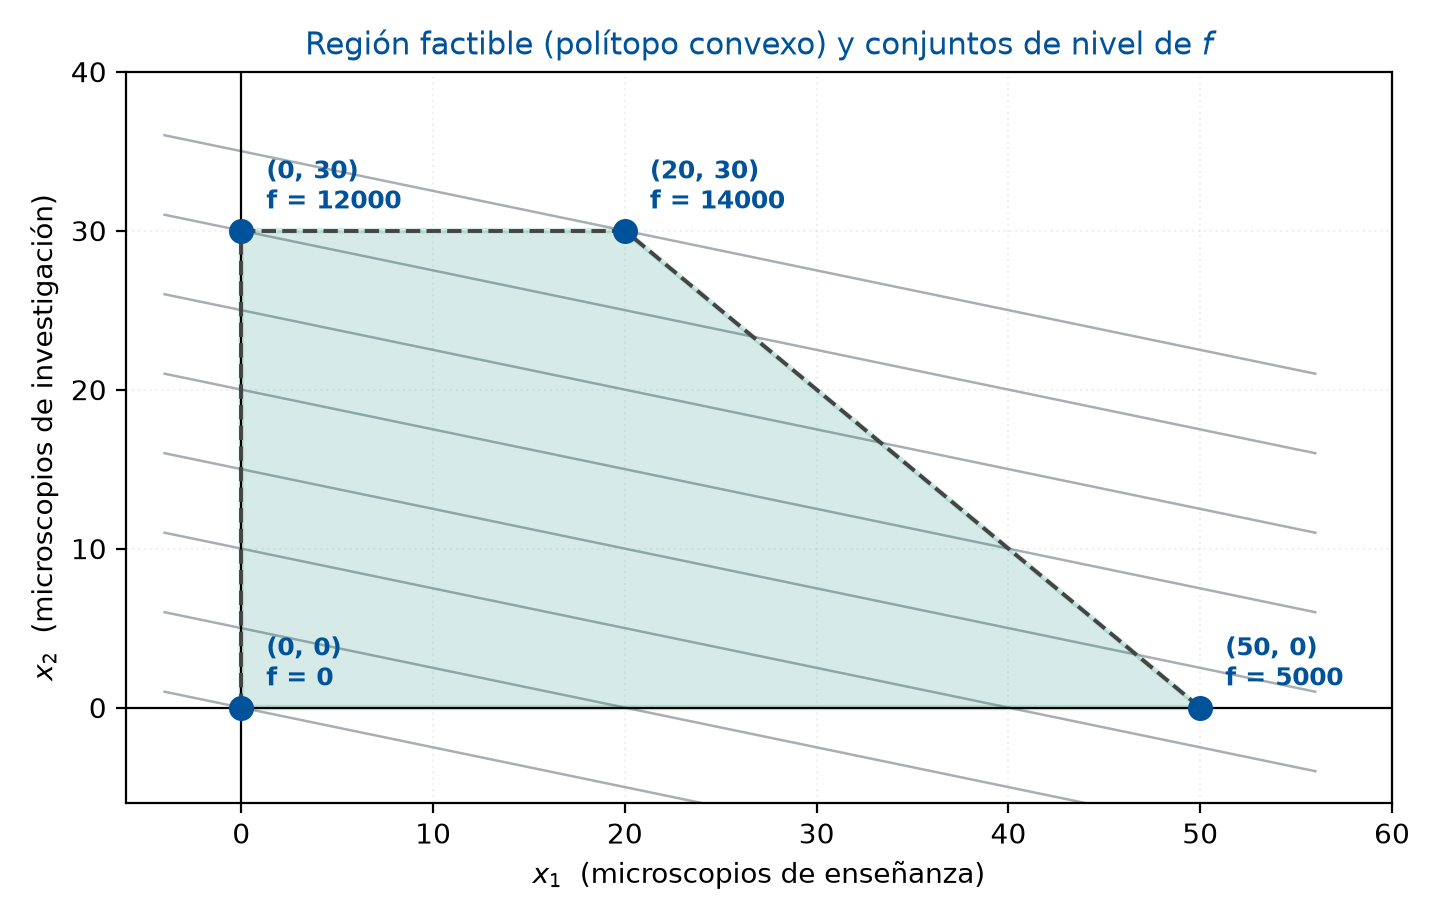
\includegraphics[width=0.70\textwidth]{images/fig_3_1_politopo.png}
  \end{figure}
  \vfill
  {\scriptsize\color{gray}
    Los conjuntos de nivel de $f$ son rectas paralelas (el gradiente es constante);
    el máximo y el mínimo tocan siempre algún vértice.}
  \fuente
\end{frame}

% =============================================================================
\section{El método simplex de Dantzig}
% =============================================================================

\begin{frame}{La idea}
  \small
  \begin{itemize}
    \item Dos propiedades bastan:
      \begin{enumerate}
        \item un extremo local ocurre en un vértice;
        \item el extremo local es global (convexidad).
      \end{enumerate}
    \item Se \textbf{camina de vértice en vértice} (\emph{pivoting}) por aristas que
      aumentan el objetivo, hasta que ninguna dirección libre mejora.
    \item El objetivo crece \textbf{monótonamente} de pivote en pivote.
    \item Cualquier variable holgada puede aumentar sin violar nada:
      su holgura es no nula.
  \end{itemize}
  \fuente
\end{frame}

\begin{frame}{Regla de pivoteo de Dantzig}
  \small
  \begin{enumerate}
      \item \textbf{Relajar una restricción activa (elegir la columna).}
      Se elige la dirección en que el objetivo más crece: la componente mayor
      del gradiente $\nabla f = c$. Esa variable tight se afloja.
    \item \textbf{Tensar una variable holgada (elegir la fila).}
      Entre las holguras candidatas se toma la que se violaría \emph{primero}
      al aumentar la variable recién aflojada: la de \textbf{menor razón $b_j/a_j$}.
    \item \textbf{Recentrar} en el nuevo vértice: se intercambian las posiciones de
      la variable aflojada y la tensada, y se sustituye la aflojada en el objetivo
      y en las demás restricciones.
  \end{enumerate}
  \vfill
  {\scriptsize\color{gray}
    Es casi idéntico a la eliminación gaussiana con pivoteo.}
  \fuente
\end{frame}

\begin{frame}{El ejemplo a mano}
  \small
  Forma con holgura (microscopios):
  \[
    s_1 = 50 - x_1 - x_2, \qquad s_2 = 30 - x_2
  \]
  \begin{itemize}
    \item \textbf{Vértice $(0,0)$}: $x_1,x_2$ tight; $s_1 = 50$, $s_2 = 30$ (holgadas).
      El gradiente $(100, 400)$ es mayor en $x_2$ $\Rightarrow$ se afloja $x_2$.
    \item Al aumentar $x_2$, la restricción $s_2 = 0$ se viola primero
      ($30/1 < 50/1$) $\Rightarrow$ se tensa $s_2$, y $x_2 = 30 - s_2$.
    \item Sustituyendo, el objetivo pasa a $\max\; 100x_1 - 400 s_2 + 12000$:
      nuevo vértice $(0,30)$, $f = 12000$.
    \item Segundo pivote: se afloja $x_1$ y se tensa $s_1$ $\Rightarrow$ vértice
      $(20,30)$, $f = 14000$. \textbf{Óptimo.}
  \end{itemize}
  \fuente
\end{frame}

\begin{frame}{El camino de vértice en vértice}
  \small
  \begin{figure}
    \centering
    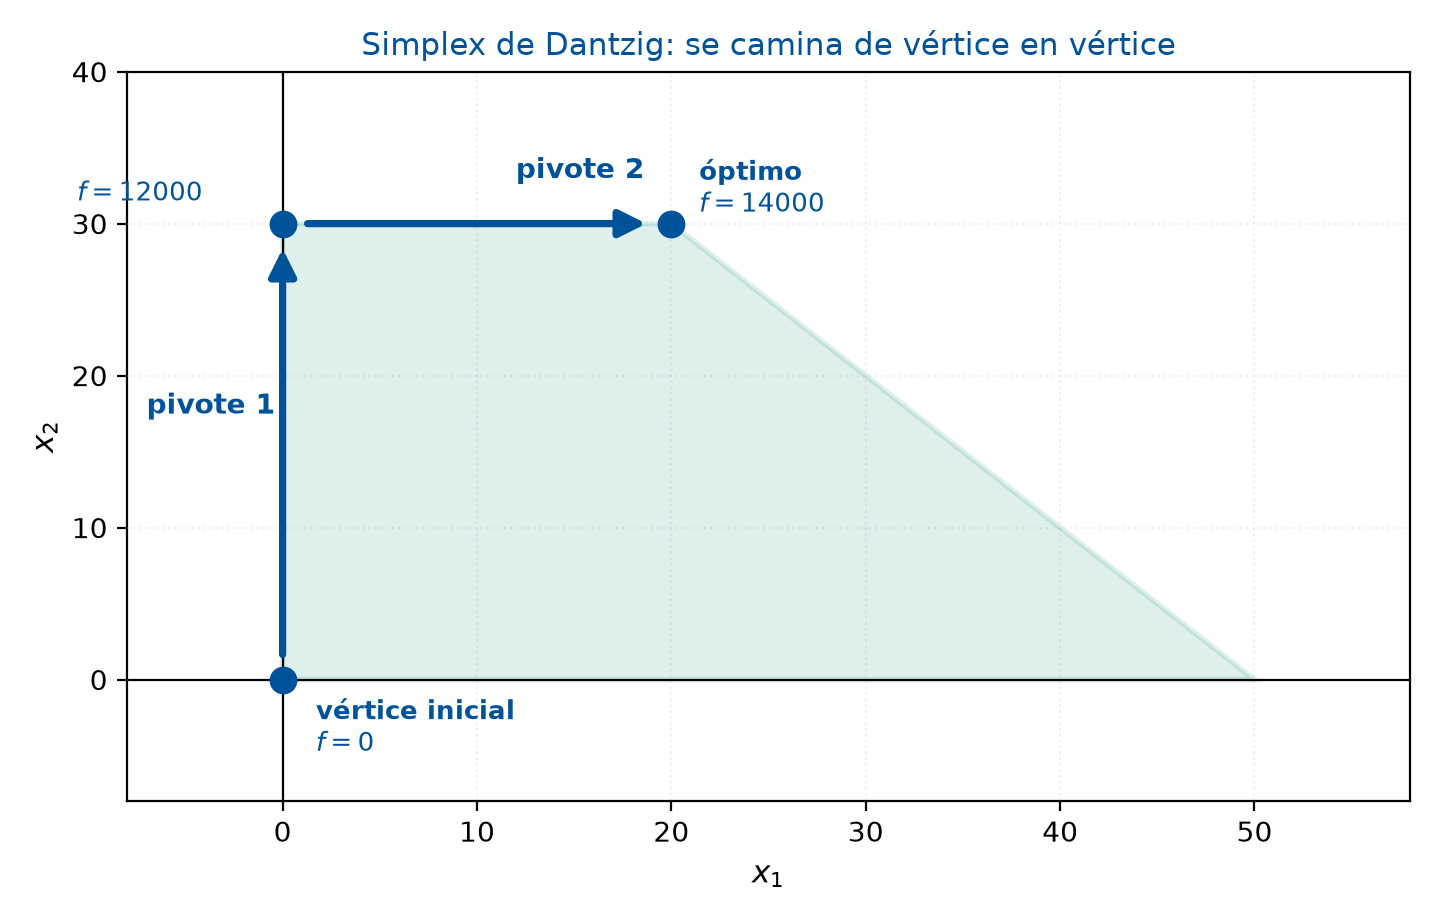
\includegraphics[width=0.72\textwidth]{images/fig_3_5_pivoteo.png}
  \end{figure}
  \vfill
  {\scriptsize\color{gray}
    Cada pivote recorre una arista del politopo; el objetivo nunca disminuye.}
  \fuente
\end{frame}

% =============================================================================
\section{El método del tableau}
% =============================================================================

\begin{frame}{Tableau simplex}
  \small
  Reescribir el PL entero en cada pivote es engorroso. El \emph{tableau} lo hace
  sistemático, con operaciones de fila tipo eliminación gaussiana:
  \[
    \begin{array}{c|cccc}
      & f & x & s & \\ \hline
      f & 1 & -c^T & 0 & 0 \\
      s & 0 & A & I & b
    \end{array}
  \]
  \begin{itemize}
    \item La \textbf{fila objetivo} codifica $f$ en términos de las variables activas.
    \item La \textbf{fila de restricciones} codifica $Ax + s = b$.
    \item La última columna lleva el valor actual de $f$ y de cada $s_i$.
    \item Es la misma operatoria que invertir una matriz:
      $\bigl[\,A \mid I\,\bigr] \to \bigl[\,I \mid A^{-1}\,\bigr]$.
  \end{itemize}
  \fuente
\end{frame}

\begin{frame}{Iteración de pivoteo}
  \small
  \begin{enumerate}
    \item \textbf{Columna a aflojar:} la variable activa con el coeficiente más
      negativo en la fila objetivo (en un problema de maximización).
    \item \textbf{Fila a tensar:} test de razón mínima, $\mathrm{RHS}/\text{coef. pivote}$
      más pequeño.
    \item \textbf{Reducción por filas} alrededor del pivote: la entrada pivote se vuelve
      $1$ y el resto de la columna, $0$.
  \end{enumerate}
  \vfill
  \begin{block}{Criterio de paro}
    Se itera hasta que \textbf{no quedan coeficientes negativos en la fila objetivo}.
    Ese vértice es óptimo local y, por convexidad, \textbf{global}.
  \end{block}
  \fuente
\end{frame}


\begin{frame}{Excepciones y casos borde}
  \small
  \begin{itemize}
    \item \textbf{Problema no acotado}: si en el test de razón mínima todos los
      coeficientes de pivote son negativos, el objetivo crece sin límite.
      Ej.: $\max x_1+x_2$ s.t.\ $2x_1 - x_2 \ge 2$, $2x_2 - x_1 \ge 2$
      (el dual es infactible).
    \item \textbf{Degeneración}: varias restricciones activas a la vez o empate en el
      test de razón $\Rightarrow$ \textbf{ciclado}. Se rompe con la
      \textbf{regla de Bland}.
    \item \textbf{Forma no estándar}: igualdades $Ax = b$ o restricciones $Ax \ge b$
      no admiten holgura directa; el simplex necesita partir de una
      \emph{solución básica factible}.
  \end{itemize}
  \vfill
  \begin{alertblock}{Phase I y Phase II}
    Se introducen \textbf{variables artificiales} $r \ge 0$ y se resuelve
    $\min 1^T r$ con $Ax + r = b$. Si el mínimo es $0$, hay solución factible y se
    pasa a \textbf{Phase II}; si es $>0$, el problema es \textbf{infactible}.
  \end{alertblock}
  \fuente
\end{frame}

% =============================================================================
\section{Dualidad}
% =============================================================================

\begin{frame}{El problema dual}
  \small
  A todo programa lineal (\emph{primal}) le corresponde otro (\emph{dual}) que acota
  su valor óptimo. La relación es una \textbf{transposición}:
  \[
    \underbrace{\max\; c^T x \quad \text{s.t.}\quad Ax \le b,\; x \ge 0}_{\text{primal}}
    \qquad\Longrightarrow\qquad
    \underbrace{\min\; b^T y \quad \text{s.t.}\quad A^T y \ge c,\; y \ge 0}_{\text{dual}}
  \]
  \begin{itemize}
    \item $c$ del primal $\to$ $b$ del dual; $b$ $\to$ $c$; $A \to A^T$.
    \item Se interpreta \emph{multiplicando} las restricciones del primal por
      $y_1, y_2, y_3$ y sumando, para acotar $c^T x$ por arriba.
  \end{itemize}
  \fuente
\end{frame}

\begin{frame}{Dualidad débil, fuerte y su gap}
  \small
  \begin{block}{Dualidad débil}
    Para todo $x$ factible del primal y todo $y$ factible del dual:
    \[
      c^T x \le b^T y
      \quad\Longrightarrow\quad
      \max_{x\in X} c^T x \;\le\; \min_{y\in Y} b^T y .
    \]
    La brecha entre ambos óptimos es el \textbf{duality gap}.
  \end{block}
  \begin{block}{Dualidad fuerte}
    Si el primal tiene solución básica factible óptima, los dos valores
    \textbf{coinciden} y el gap es cero. Cada solución factible de un problema
    \emph{certifica} la optimalidad del otro.
  \end{block}
  \begin{itemize}
    \item $y_j$ = multiplicador de Lagrange de la restricción $j$:
      \textbf{precio sombra} o \textbf{valor marginal}.
    \item Mide la sensibilidad del valor óptimo ante cambios en $b$ y en $c$.
    \item Los métodos de punto interior resuelven primal y dual simultáneamente.
  \end{itemize}
  \fuente
\end{frame}

% =============================================================================
\section{Programación entera}
% =============================================================================

\begin{frame}{Programación lineal entera (ILP)}
  \small
  \[
    \max_x\; c^T x \quad \text{s.t.}\quad Ax \le b,\qquad x \in \{0,1\}^n \;\text{o}\; \mathbb{N}^n
  \]
  \begin{itemize}
    \item Variables enteras: decisiones de sí/no (empaque, ubicación, inclusion).
    \item Muchos ILP son \textbf{NP-hard}: no se conoce algoritmo polinomial en el
      peor caso.
    \item \textbf{Relajación LP}: se permiten $x$ continuas $\ge 0$.
      Toda solución entera factible es factible para la relajación, luego la
      relajación da una \textbf{cota superior} del óptimo entero.
    \item Si el óptimo de la relajación ya es entero, \emph{es} el óptimo del ILP.
    \item En el ejemplo de los microscopios los vértices eran enteros: PL e ILP
      coinciden.
  \end{itemize}
  \fuente
\end{frame}

\begin{frame}{Branch-and-bound y planos de corte}
  \small
  \begin{columns}[T,onlytextwidth]
    \begin{column}{.48\textwidth}
      \textbf{Branch-and-bound}
      \begin{itemize}
        \item Se resuelve el PL relajado.
        \item Para cada $x_j$ no entera se crea un subproblema con
          $x_j \le \lfloor x_j \rfloor$ y otro con $x_j \ge \lceil x_j \rceil$.
        \item Si la cota de un subproblema es peor que una solución entera
          conocida, esa rama se \textbf{poda}.
        \item Construye un árbol de búsqueda.
      \end{itemize}
    \end{column}
    \begin{column}{.48\textwidth}
      \textbf{Planos de corte}
      \begin{itemize}
        \item Se agregan restricciones lineales (\emph{cortes}) que eliminan
          soluciones no enteras y conservan todos los enteros factibles.
        \item Cada corte estrecha la región factible hacia el
          \emph{casco entero}.
        \item Tipos: de Gomory, \emph{cover cuts}, desigualdades de cliques.
      \end{itemize}
    \end{column}
  \end{columns}
  \vfill
  \begin{block}{En la práctica}
    La mayoría de los solvers usa un enfoque híbrido \textbf{branch-and-cut}:
    la estructura de búsqueda global del B\&B con cortes que reducen la ramificación.
  \end{block}
  \fuente
\end{frame}

\begin{frame}{Relajación LP frente al óptimo entero}
  \small
  \begin{figure}
    \centering
    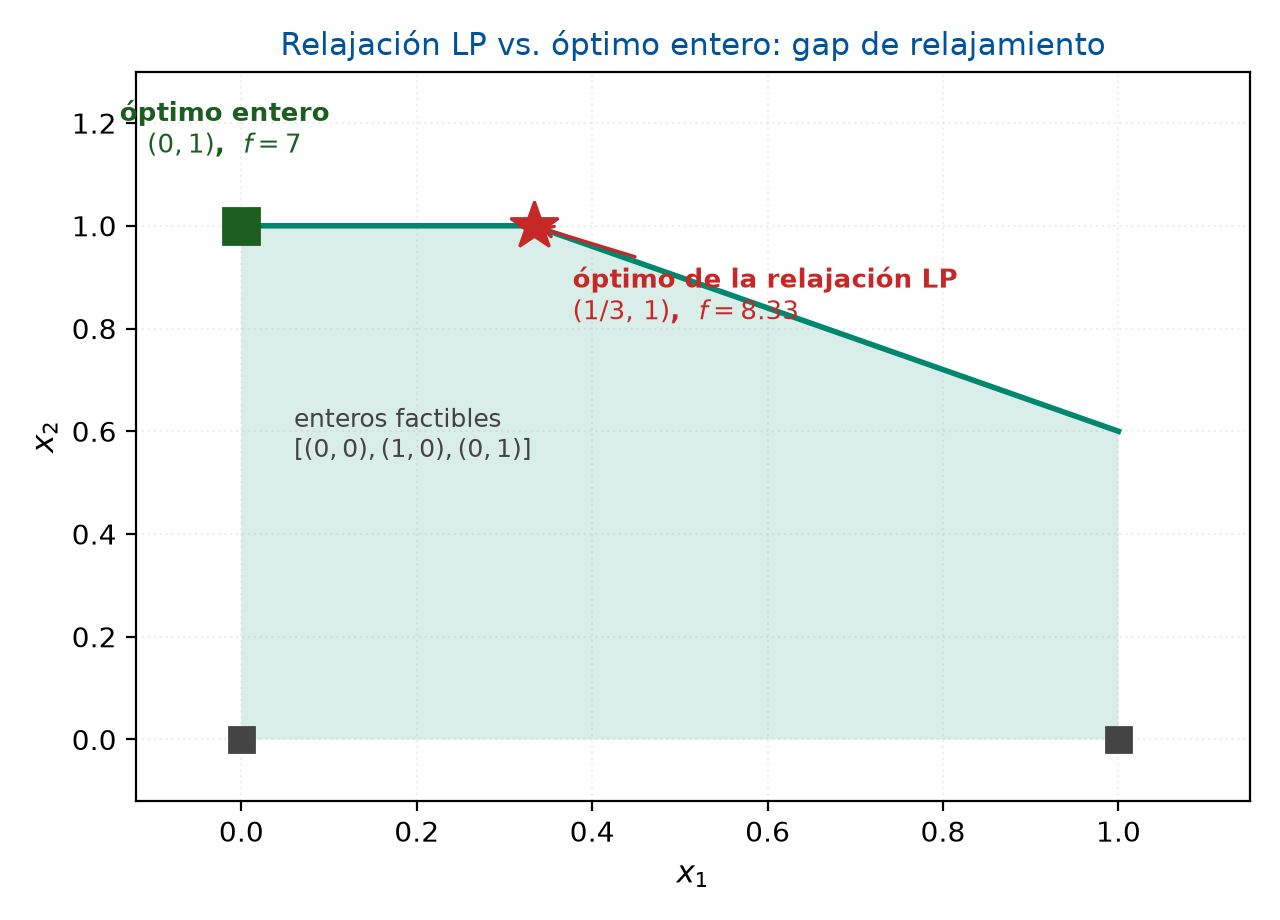
\includegraphics[width=0.46\textwidth]{images/fig_3_8_relajacion.png}
  \end{figure}
  \vfill
  {\scriptsize\color{gray}
    El óptimo de la relajación es una cota superior del entero; si es fraccionario,
    no se puede aceptar como solución.}
  \fuente
\end{frame}

\begin{frame}{Dos problemas clásicos}
  \small
  \textbf{Problema de la mochila (knapsack)} --- NP-hard:
  \[
    \max_{x_j\in\{0,1\}}\; \sum_{j=1}^n p_j x_j
    \quad \text{s.t.}\quad \sum_{j=1}^n w_j x_j \le W
  \]
  \begin{itemize}
    \item Prototipo de la asignación de recursos: empaque de cajas, calendarización
      de tareas, reparto de presupuesto.
    \item $2^n$ subconjuntos: la enumeración es exponencial.
    \item Panel 3.3 del libro: con \texttt{pulp} y con fuerza bruta se obtiene la
      misma solución óptima (ítems 1, 2, 5, 6; peso 20; valor 81).
  \end{itemize}
  \textbf{Agente viajero (TSP)} --- NP-hard:
  \[
    \min_{x_{ij}\in\{0,1\}}\; \sum_{(i,j)\in E} c_{ij} x_{ij}
    \quad \text{s.t.}\quad \textstyle\sum_j x_{ij}=1 \;\forall i,\quad
    \sum_i x_{ij}=1 \;\forall j
  \]
  \begin{itemize}
    \item Una sola ruta que visite cada ciudad exactamente una vez y regrese al inicio.
    \item Requiere restricciones adicionales para eliminar los \emph{sub-tours}.
    \item Se combina con geometría: empaque en planta, layout de almacén,
      \textbf{diseño de chips VLSI}.
  \end{itemize}
  \fuente
\end{frame}

% =============================================================================
\section{Cierre}
% =============================================================================

\begin{frame}{Puntos para recordar}
  \small
  \begin{enumerate}
    \item La PL es convexa: el óptimo está en un vértice y es global.
    \item Las \textbf{variables de holgura} traducen "activa/inactiva" a "$s_i=0$ /
      $s_i>0$": esa notación es la que hace posible el simplex.
    \item El simplex \textbf{camina de vértice en vértice}; el tableau es su
      implementación matricial (pivoteo tipo gaussiana).
    \item Excepciones a vigilar: no acotado, degeneración (ciclado) y forma no
      estándar (Phase I).
    \item La \textbf{dualidad} da cotas y certificados de optimalidad; $y$ son
      precios sombra.
    \item La programación entera es NP-hard; la relajación LP acota y el
      branch-and-cut resuelve.
  \end{enumerate}
  \vfill
  \begin{alertblock}{Idea final}
    La PL es notable porque combina una geometría limpia (politopos, vértices)
    con un algoritmo exacto y enumerable, y sirve de banco de pruebas para
    dualidad, optimalidad y enteros.
  \end{alertblock}
\end{frame}

\begin{frame}{Para profundizar}
  \small
  \textbf{Textos}
  \begin{itemize}
    \item Dantzig, \emph{Linear Programming and Extensions}, 1963.
    \item Bertsimas y Tsitsiklis, \emph{Introduction to Linear Optimization}, 1997.
    \item Wolsey y Nemhauser, \emph{Integer and Combinatorial Optimization}, 2014.
    \item Schrijver, \emph{Theory of Linear and Integer Programming}, 1998.
    \item Hillier y Lieberman, \emph{Introduction to Operations Research}, 2021.
    \item Korte y Vygen, \emph{Combinatorial Optimization}, 2018.
    \item Martello y Toth, \emph{Knapsack Problems}, 1990.
  \end{itemize}
  \textbf{Artículos}
  \begin{itemize}
    \item Dantzig, \emph{Maximization of a linear function of variables subject to
      linear inequalities}, 1951.
    \item Karmarkar, \emph{A new polynomial-time algorithm for linear programming}, 1984.
    \item Gomory, \emph{Outline of an algorithm for integer solutions to linear
      programs}, 1960.
  \end{itemize}
  \vfill
  \begin{center}
    \large\textbf{¿Preguntas?}
  \end{center}
\end{frame}

\end{document}
